\chapter{Research Background}

%citazione introduttiva
\epigraph{\textit{The line between statistics, computer science and engineering is getting thinner.}}{}


This chapter reviews the relevant literature identifying the academic position of this work. As introduced, this work provides advances in the field of engineering applied to the “system analysis” (see Figure \ref{fig_operationsResearch}) of a supply chain by using data-driven technologies.\par

Before starting with this data-driven journey, it is necessary to introduce a brief glossary with the keywords used to gather academic papers by scholars and practitioners (see Table \ref{tab_dataGlossary}).

% INSERT tab_dataGlossary
\begin{figure}[hbt!]
\centering
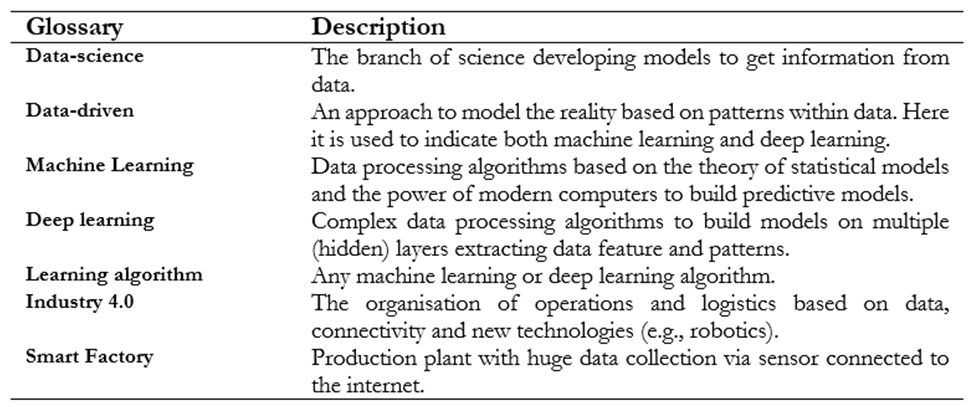
\includegraphics[width=0.9\textwidth]{SectionIntroduction/researchBackground_figures/tab_dataGlossary.png}
\captionsetup{type=figure}
\caption{Glossary of data science terms.}
\label{tab_dataGlossary}
\end{figure}

\section{Academic background}

The data-driven approach is gathering an increasing interest in literature during the last decade. In particular, the number of research paper approaching logistics research issues from a data-driven perspective is increasing exponentially ~\cite{Moktadir2019, Spanaki2018}. Figure \ref{fig_literature_trend} illustrates research trends on Scopus reporting the number of research papers published in international journals resulting from four research queries. The world “machine learning”, “deep learning” and “data-driven” are used together with the word “industry” to check how literature evolves approaching this topic from an industrial perspective. The last trend is focused on the field of supply chain management. This trend is similar, but with a lower absolute number of papers.

% INSERT fig_literature_trend
\begin{figure}[hbt!]
\centering
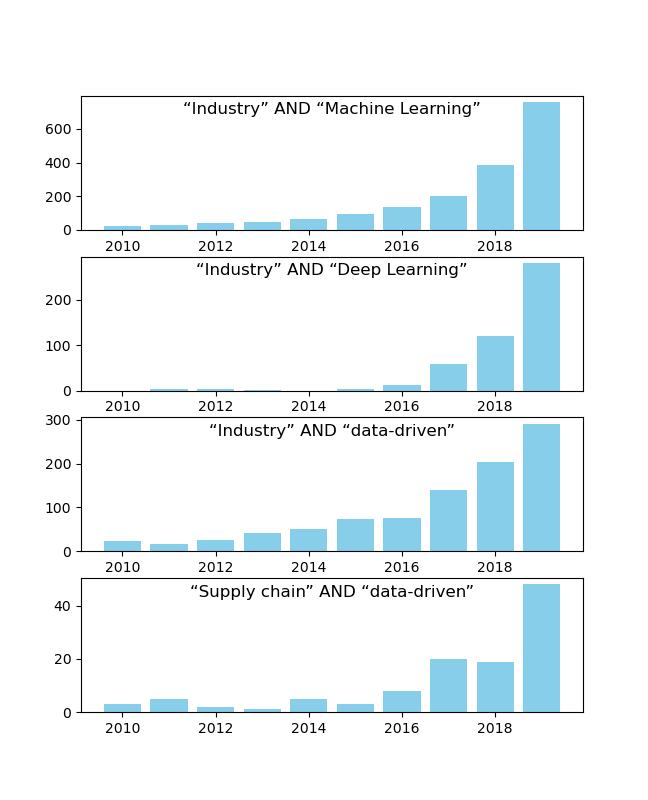
\includegraphics[width=0.9\textwidth]{SectionIntroduction/researchBackground_figures/fig_literature_trend.png}
\captionsetup{type=figure}
\caption{Literature trends corrsemponding to different research queries on Scopus.}
\label{fig_literature_trend}
\end{figure}

This analysis shows that, in the last few years, scholars are paying more attention to data-driven approaches applied to industrial fields. Nevertheless, the amount of contributions in the field of industrial engineering and supply chain is still limited. A closer investigation of the industrial engineering field confirms the need for a broader study of data-driven methods in this field ~\cite{Nguyen2018}. Figure \ref{fig_literature_pie} categorises the topic of industrial engineering approached with a data-driven approach in a sample of 23 journal articles.

% INSERT fig_literature_pie
\begin{figure}[hbt!]
\centering
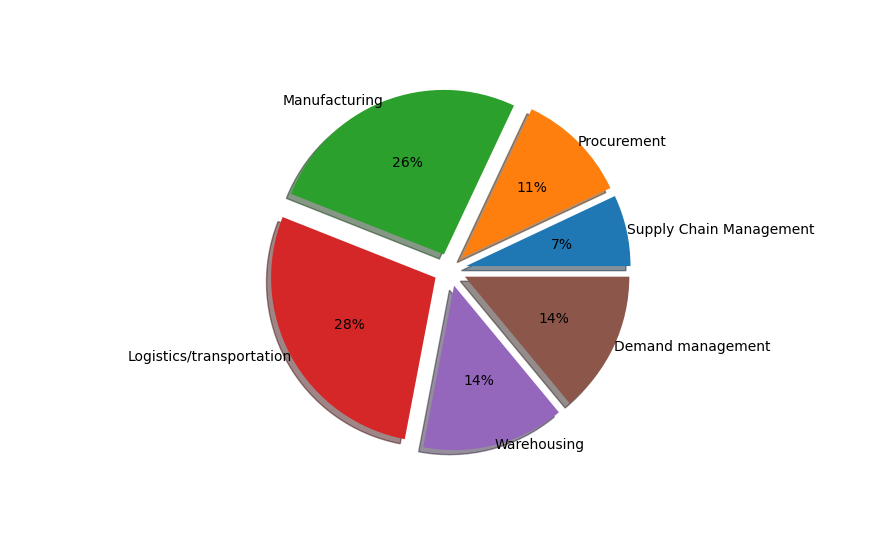
\includegraphics[width=0.9\textwidth]{SectionIntroduction/researchBackground_figures/fig_literature_pie.png}
\captionsetup{type=figure}
\caption{Fields of application of data-driven algorithms in the industrial engineering sector.}
\label{fig_literature_pie}
\end{figure}

Industrial engineering shares engineering and decision science features. Figure \ref{fig_topics_pie} (defined on a sample of 52 journal articles) shows that both of them are areas of research where analytics and data-driven modelling are established methodologies ~\cite{Gupta2019}.

% INSERT fig_topics_pie
\begin{figure}[hbt!]
\centering
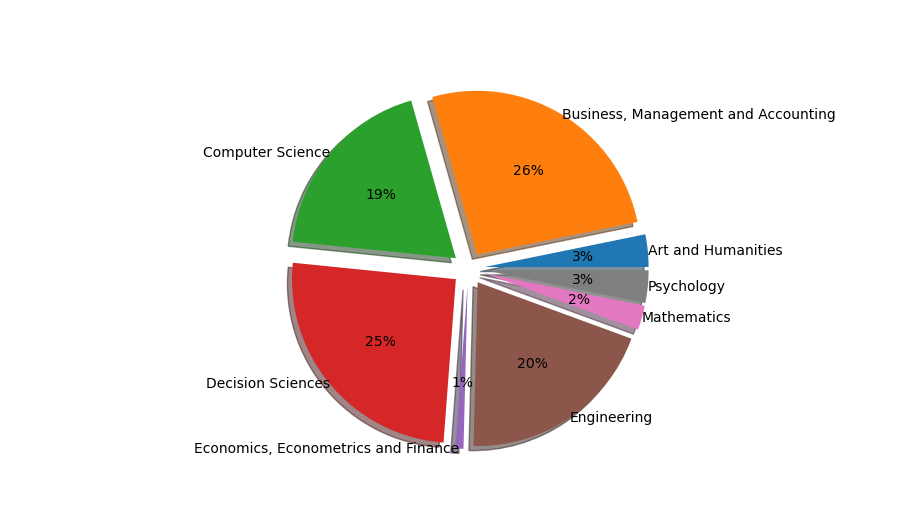
\includegraphics[width=0.9\textwidth]{SectionIntroduction/researchBackground_figures/fig_topics_pie.png}
\captionsetup{type=figure}
\caption{The fields of application of data-driven algorithms.}
\label{fig_topics_pie}
\end{figure}

The literature lacks a comprehensive approach of data-driven models in the field of logistics research as tools for system analysis ~\cite{Wang2016, Lamba2018}. Many papers show frameworks for the application of analytics and data-driven methods to sub-topics as safety engineering, industrial database design data structures and real-time data collection with internet-of-things (IoT) industrial devices ~\cite{Huang2018, Zhang2018}. Nevertheless, none of them proposes a holistic point of view on logistics and operations.\par

On the other side, they clearly recognise a value behind data ~\cite{Balandin2015, Uckelmann2008} and the importance of smart logistics and smart factory whose capability is to adapt decision making dynamically to predict future scenarios.\par

This new approach involves a large mass of data exchanged between several actors ~\cite{Kawa2012, Singh2017}. Literature suggests robust methodologies to manage the information flow of data ~\cite{Tran-Dang2018}. The outcome of these data structures supports the development of the smart factory, i.e. a manufacturing plants where information is used to control the process and to make decisions on the future processes (i.e. the design) ~\cite{Hajdul2011}. \par

In ~\cite{TAN2018}, they identify three main research issues to improve the operation in a smart factory using data-driven methods:

\begin{enumerate}
    \item modelling the theory and method of smart factory;
    \item knowledge discovery and knowledge management based on industrial big data analysis;
    \item adaptive scheduling and optimisation of the smart factory.

\end{enumerate}

This book focuses on the key issues (2) and (3). Often, literature focuses only on theoretical frameworks for the application of data-driven methods ~\cite{DaSilva2019}. In this work, we aim at a comprehensive approach for logistics and operations being practice-ready for a company proposing areas of application of data-driven methods.

\section{Industrial background}
In addition to the academic relevance, we want to highlight the rationale of this work considering the structure of the external industrial sector: data science is the present, not the future. In the last decade, companies started creating a new professional role called “data scientist” able to generate value from industrial data. From this perspective, the statistic is the history, machine learning is the past, and deep learning is the present ~\cite{HubSpot2016}. These methodologies have already been established and implemented in many business areas (e.g. marketing, finance) with or without the contribution of the research community since a number of companies recognised their data could be used to improve the efficiency, reliability and sustainability of their business ~\cite{Nascimento2019, Trkman2010}.\par

Looking at the industrial practice, we notice that there is an enormous potential for data-driven application in the field of logistics. The industry is reacting to this new trend with significant investments in data-driven projects ~\cite{Worldeconomicforum2017, Zhong2016}. Managers and directors from logistics and operations identify in the big data analytics the main tool to handle decision and processes in the future ~\cite{Rossmann2018}. Nevertheless, a significant gap exists between large companies, able to train data scientist themselves, and small and medium enterprises (SME) which cannot afford this kind of investment ~\cite{Dubey2019}.\par

It is the case of large third-party providers that develop machine learning and artificial intelligence tools to support their business ~\cite{Ku2018}. They identify a precise workflow to check if a data-driven approach can be used to generate value, improving a logistic process (see Figure \ref{fig_applicationML}) with two main activities:

\begin{enumerate}
    \item creating new knowledge;
    \item reducing costs.

\end{enumerate}

% INSERT fig_applicationML
\begin{figure}[hbt!]
\centering
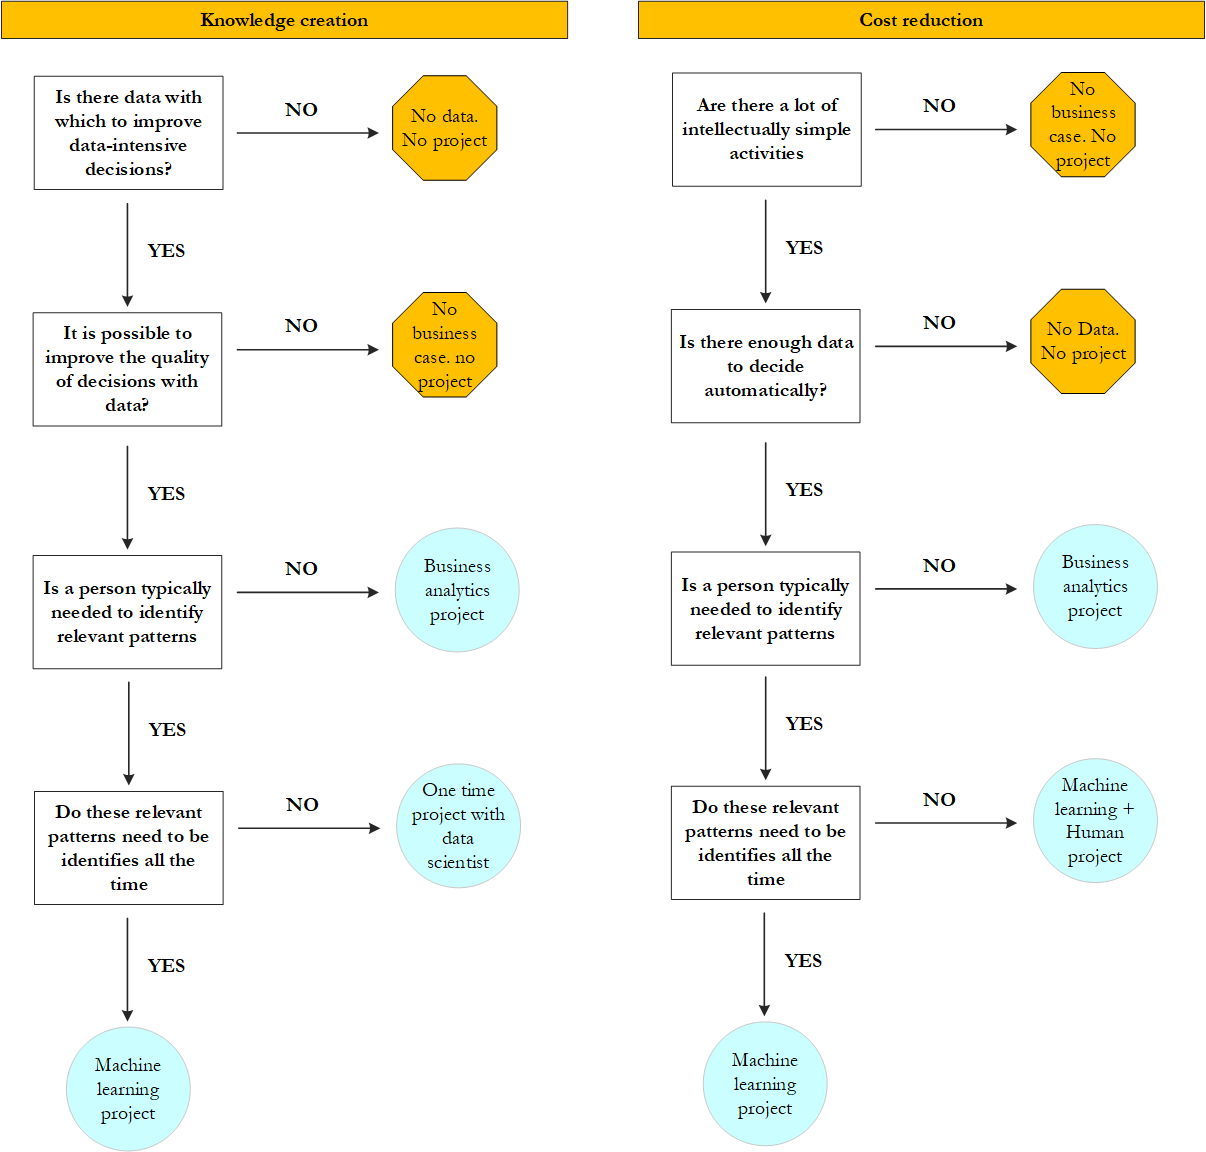
\includegraphics[width=0.9\textwidth]{SectionIntroduction/researchBackground_figures/fig_applicationML.png}
\captionsetup{type=figure}
\caption{Checklist for the implementation of a data-driven project adapted from ~\cite{Ku2018}.}
\label{fig_applicationML}
\end{figure}

These two objectives are the reason why companies started collecting data on their processes and hiring data scientists. The flowcharts in Figure \ref{fig_applicationML} identify the necessary ingredients to get success from data-driven approach. The quantity and quality of the data is, obviously, a crucial issue to work with a data-driven approach. Besides, the data collected must be relevant to solve a decision problem. Finally, if an algorithm can find patterns better than a human does, the data-driven approach is a good choice to create knowledge and reduce costs.\par

Both these objectives are reachable when data scientists have both analytic skills and profound knowledge of the industry-specific domain ~\cite{Ku2018}. When these two characteristics come together, data-driven application leads these companies to success while some small logistics companies still strive to work with pen and paper.

Logistics companies identify the need to anticipate the behaviour of the market with predictions on:

\begin{itemize}
    \item lead times;
    \item transport capacity;
    \item customer orders. 

\end{itemize}

Predictive logistics can forecast the value of these metrics anticipating market demand. Traditional logistics is way less efficient and unable to anticipate market behaviour ~\cite{LOGISTICAEFFICIENTE2019}. Data-driven tools are not limited to transportation activities.  Recent applicationS in the manufacturing and storage industry have seen several predictive models to support the operations ~\cite{Logisticofthings2017, Package.ai2017, Reporter2016}.\par

While a small number of big companies recognises the value of its operational data, researchers strive to get data to test their assumptions enriching the literature and public knowledge. Besides, the more these companies see a profit in their data-driven approaches, the less they are willing to share data with the research community. This happens because they get a competitive advantage from the utilisation of their data and sharing their valuable knowledge with the public would not be safe for their business.\par

In this sense, our work is even harder since it is difficult not only to design new methods but also to get data to test them and keep them useful in the real world. For this reason, we notice a gap between practice and academic research, especially when internal research units of multinational companies hold the data and autonomously lead the research activities.\par

Also, the application of data-driven models in industrial practice is still limited in the field of logistics and operations ~\cite{Garver2019}. We think that academic research has the responsibility to explore the role and the potential of analytics and data-driven methods in the logistics and operations fields.\par

%\clearpage
\bibliographystyle{ieeetr}
\bibliography{SectionIntroduction/researchBackground_ref}
